%!TEX root = thesis.tex
\chapter{Introduction}
\label{cha:introduction}

Ever since the dawn of time, the humankind have looked at the stars and wondered if we are alone in
this Universe. To answer this question, one must look toward the field of extrasolar planets
(exoplanets). This is a rapidly growing field in astronomy and science in general. Since the first
confirmed discovery of an exoplanet around a millisecond pulsar in 1992 by \citet{Wolszczan1992} and
three years later, the more interesting exoplanet 51 Peg b discovered around a solar-type star by
\citet{Mayor1995}, more than 3600 exoplanets have been discovered at the time of writing, July
2017\footnote{\url{http://exoplanet.eu/}}.

With the discoveries of exoplanets, the main focus is now mainly on finding the twin of Earth, that
is a planet that can harbour life as we know it. However, it is not enough to simply discover small
rocky exoplanets. Accurate and precise determination of the stellar parameters are crucial as the
planetary parameters (radius, mass, bulk density, etc.) are directly derived from their host's
parameters.

In this chapter there will be a general introduction to exoplanets, detection methods, and
characterisation (\sref{sec:exoplanets}). Then a throughout introduction on the exoplanet host
stars (\sref{sec:planet_host_stars}), which is the main focus on this thesis. While learning about
host stars, and stars in general, the results have wide-spread applications, where some will briefly
be discussed in the end of this chapter (\sref{sec:stars_application}) before an introduction on
what this thesis will consists of (\sref{sec:this_thesis}).



\section{Exoplanets}
\label{sec:exoplanets}

The holy grail in the field of exoplanets is to find the first exoplanet with life. This is by no
means an easy task. To give an idea of the difficulty of detecting life on an exoplanet, one must
understand all the difficulties to simply detect and confirm an exoplanet. This will shortly be
described in the sections below

\subsection{Detecting exoplanets}
\label{sec:detecting_exoplanets}

There are sex ways of detecting exoplanets, some with advantages over others. In combination with
each other, one can potentially learn a lot about the exoplanet(s).

It is important to note, that different things might mimic planetary signals, however they will not
be described in this thesis. The confirmation of an exoplanet often happen, when two techniques are
able to detect the same exoplanet.



\subsubsection{Transit method}

The most successful method, if based on numbers of exoplanets detected, is the transit method. This
is a well-known method in astronomy, however only used in the last decade for detecting exoplanets.
Before this, it has been used extensively for finding and characterising binary stars. The
difference here is, that the exoplanet does not radiate (or at least very little radiation). An
example of an exoplanet transiting a star can be seen in \fref{fig:transitMethod}.

\begin{figure}[htpb!]
    \centering
    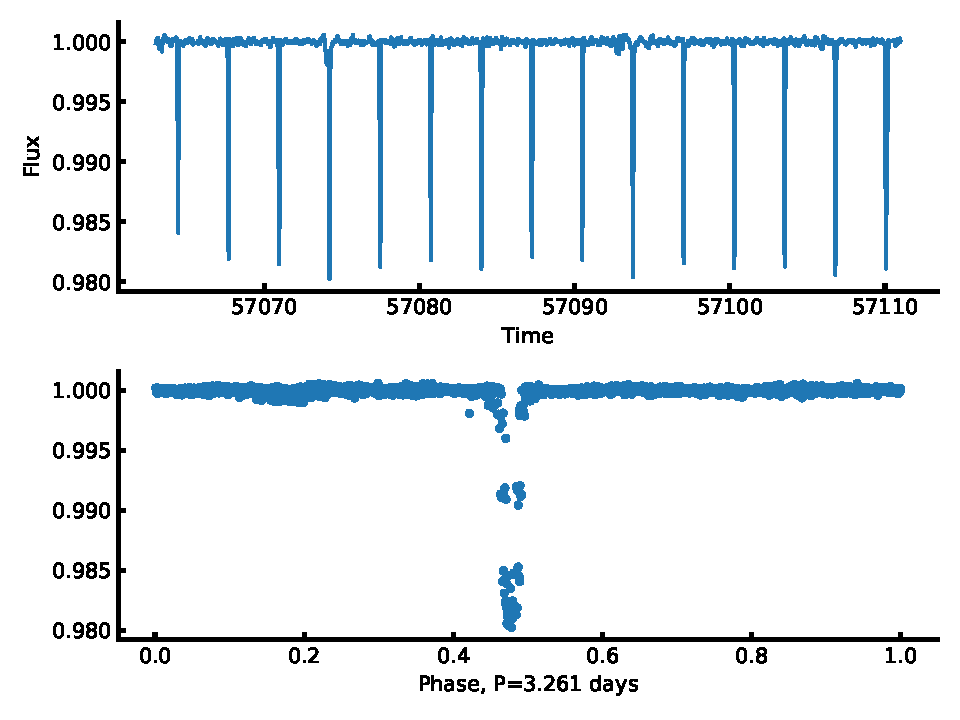
\includegraphics[width=1.0\linewidth]{figures/transitMethod.pdf}
    \caption{\emph{Upper plot}: The lightcurve of a star with an exoplanet transiting.
             \emph{Lower plot}: The phase curve of the above lightcurve.}
    \label{fig:transitMethod}
\end{figure}

As an exoplanet orbit a star, it might transit its host as seen from an observer here on Earth. This
signal might be detected if the star's brightness is being monitored as a periodic signal. The
decrease in brightness as the planet transit the star is directly related to ration between the
stellar radius $R_\ast$ and the planetary radius $R_p$:
\begin{align}
  k = \sqrt{\frac{R_p}{R_\ast}},
\end{align}
where $k$ is the depth of the transit compared to the total stellar brightness.

It is possible to obtain the radius of an exoplanet with this method. However, detailed analysis of
the phase curve of an exoplanet can reveal the surface temperature of the exoplanet. The transit
described above is also known as the primary transit. If it is possible to detect the secondary
transit, that is when the exoplanet goes behind the star as seen from Earth, the difference in light
(planet + star right before secondary transit compared to just star) gives the flux of the planet
and thus the surface temperature. This is a difficult task as secondary transits are intrinsic
faint.


\subsubsection{Radial velocity method}

The radial velocity method is the indirect study of the motion of the host star using the Doppler
effect caused by an orbiting exoplanet. This together with the transit method described above is by
far the most successful methods to detect and characterise exoplanets. The periodic signal created
by the exoplanet on the host star depends on the mass ratio between the star $M_\ast$ and the planet
$M_p$:
\begin{align}
  K = \frac{\SI{28.4329}{km/s}}{\sqrt{1-e^2}} \frac{M_p\sin i}{\Mjup} \left( \frac{M_\ast+M_p}{M_\odot} \right)^{-2/3} \left(\frac{P}{\SI{1}{year}}\right)
\end{align}
where $K$ is the semi-amplitude of the sinusoidal, $e$ is the eccentricity, $i$ is the inclination,
$P$ is the orbital period, and $\Mjup$ is the mass of Jupiter. Since $M_\ast \gg M_p$, the term
$M_\ast+M_p\simeq M_\ast$ in order to simplify the equation. Often a circular orbit is assumed,
$e=0$. The sinusoidal motion of the star can be seen in \fref{fig:rvmethod} where both the time
series and the phase curve is presented for an exoplanet.

\begin{figure}[htpb!]
    \centering
    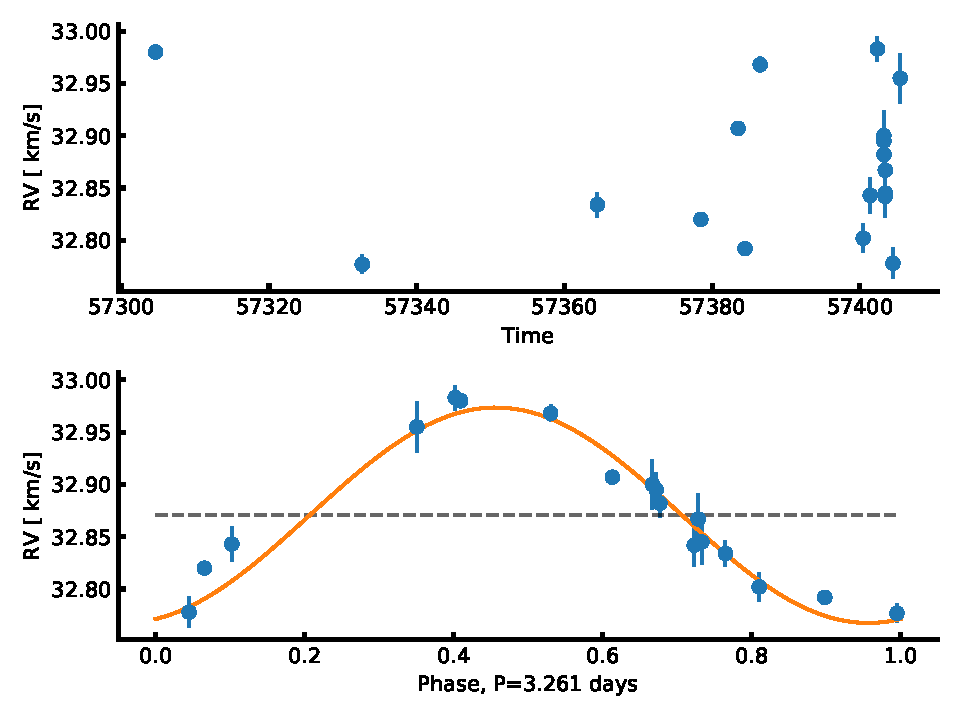
\includegraphics[width=1.0\linewidth]{figures/RVmethod.pdf}
    \caption{\emph{Upper panel}: RV time series of EPIC 9792 from the SOPHIE spectrograph.
             \emph{Lower panel}: Phase curve of the time series above, using the period of
             \SI{3.261}{days}.}
    \label{fig:rvmethod}
\end{figure}

In order to apply the radial velocity method for detecting exoplanets, it is necessary to collect
spectra, high resolution but often not high S/N, in order to cover most part of the phase of the
orbit. These spectra are often combined after the detection of the exoplanet, in order to increase
the S/N. This combined spectrum can then be used for characterising the host star.

This method is sensitive to close-in massive exoplanets, also known as hot Jupiters. In combination
with the above mentioned transit method, the mass and radius of an exoplanet can be derived, and
thus the bulk density which might give hints of the structure and composition of the exoplanet.


\subsubsection{Direct imaging}

Direct imaging is probably the easiest method to understand, however it is quite difficult to
actually use this technique. In its core, one has to carefully block the light of a star, and
directly imaging the exoplanets around it. However, it is extremely difficult to block the light of
the host star and find the reflected light of the exoplanet(s) in orbit.

This technique are sensitive to exoplanets which reflect a lot of light, i.e. a high albedo, and in
wide orbits as they are less contaminated by the residual starlight.

\subsubsection{Astrometry}



\subsubsection{Transit timing variation}



\subsubsection{Microlensing}




\section{Planet host stars}
\label{sec:planet_host_stars}

With the present diversity of exoplanets it becomes increasingly important to get an accurate and
precise characterisation of the planets in order to study them in samples and on an individual
level. An accurate and precise characterisation can give us an idea whether the planet is rocky,
composed of water or gaseous.



\section{Applications from knowing the stars}
\label{sec:stars_application}





\section{This thesis}
\label{sec:this_thesis}
